%%%%%%%%%%%%%%%%%%%%%%%%%%%%%%%%%%%%%%%%%
% English Beamer Presentation LaTeX Template
% Version:1.0 (2024.08.21)
% Author:ZJW
% Compilor:XeLaTeX
%%%%%%%%%%%%%%%%%%%%%%%%%%%%%%%%%%%%%%%%%

%----------------------------------------------------------------------------------------
%   Cover and Global Configuration
%----------------------------------------------------------------------------------------
\documentclass[12pt, aspectratio=169]{beamer} 
%%%%%%%%%%%%%%%%%%%%%%%%%%%%%%%%%%%%%%%%%
% 中文简体模板
% 版本:1.0 (2024.08.21)
% 修改者:ZJW
% 编译器:XeLaTeX
%%%%%%%%%%%%%%%%%%%%%%%%%%%%%%%%%%%%%%%%%

%----------------------------------------------------------------------------------------
%	封面及全局配置
%----------------------------------------------------------------------------------------
\usepackage{fontspec} 
%----------------------------------------------------------------------------------------
%	中文字体 (选择其中1个)
% 
% 	AutoFakeBold=3.5: 粗体的深度
% 	AutoFakeSlant=0.2: 斜体的深度
% 	Path = fonts/: 字体的路径
%----------------------------------------------------------------------------------------
\usepackage{xeCJK}
% \setCJKmainfont[AutoFakeBold=3.5 , AutoFakeSlant=0.2, Path = fonts/]{cwTeX_圓體.ttf}
% \setCJKmainfont[AutoFakeBold=3.5 , AutoFakeSlant=0.2, Path = fonts/]{SIMHEI.ttf} % 黑体
% \setCJKmainfont[
%     Path=fonts/, % 字体文件所在路径
%     BoldFont=MSYHBD.ttc, % 粗体
%     ItalicFont=MSYH.ttc, % 斜体(微软雅黑不区分斜体,所以用常规字体代替)
%     SlantedFont=MSYH.ttc, % 斜体(如果需要,可以设置与常规字体一致)
%     BoldItalicFont=MSYHBD.ttc, % 粗斜体(如果需要,可以设置与粗体一致)
%     AutoFakeBold=3.5, % 自动加粗
%     AutoFakeSlant=0.2 % 自动倾斜
% ]{MSYH.ttc} % 微软雅黑
% \setCJKmainfont[AutoFakeBold=3.5 , AutoFakeSlant=0.2, Path = fonts/]{华文行楷.ttf} 
\setCJKmainfont[AutoFakeBold=3.5 , AutoFakeSlant=0.2, Path = fonts/]{SIMSUN.ttc} % 宋体
% \setCJKmainfont[AutoFakeBold=3.5 , AutoFakeSlant=0.2, Path = fonts/]{SIMKAI.TTF} % 楷体
\XeTeXlinebreaklocale "zh" % 這兩行用來調整中文自動換行
\XeTeXlinebreakskip = 0pt plus 1pt

%----------------------------------------------------------------------------------------
%	英文字体 (选择其中1个)
% 
%----------------------------------------------------------------------------------------
% \usefonttheme{serif} % 使用 serif 字體
\setmainfont[
    Path=fonts/,
    UprightFont=TIMES.TTF,
    BoldFont=TIMESBD.TTF,
    ItalicFont=TIMESI.TTF,
    BoldItalicFont=TIMESBI.TTF
]{Times New Roman} % Times New Roman

\usepackage{color} 
%% 自定义颜色
\definecolor{JLUPurple}{RGB}{102,8,116}
\definecolor{JLUGreen}{RGB}{0,166,82}
\definecolor{JLURed}{RGB}{157,41,51}
\definecolor{JLUBlue}{RGB}{0, 0, 128}

\usepackage{mathtools, amsmath, amsfonts, amsthm, latexsym} 
\usepackage{newtxtext,newtxmath}
\usepackage[justification=centering]{caption} 
\setbeamertemplate{caption}[numbered]
\captionsetup[figure]{font=small, labelfont=md}
\captionsetup[table]{font=small, labelfont=md}
\usepackage{graphicx}  
\usepackage{booktabs}
\usepackage{subfigure} 
\usepackage{multirow} 
\usepackage{array}
\usepackage{enumerate} 
\usepackage{tikz}
\usepackage{natbib}
\usepackage{comment}
\renewcommand{\figurename}{图} 
\renewcommand{\tablename}{表} 

%----------------------------------------------------------------------------------------
%	排版形式 (选择其中1个)
%----------------------------------------------------------------------------------------

\mode<presentation>{
% \usetheme{default} 
% \usetheme{AnnArbor}  
% \usetheme{Antibes}
% \usetheme{Bergen}
% \usetheme{Berkeley}
% \usetheme{Berlin}
% \usetheme{Boadilla}
% \usetheme{CambridgeUS}
% \usetheme{Copenhagen}
\usetheme{Darmstadt}
% \usetheme{Dresden}
%\usetheme{Frankfurt}
%\usetheme{Goettingen}
%\usetheme{Hannover}
%\usetheme{Ilmenau}
%\usetheme{JuanLesPins}
%\usetheme{Luebeck}
% \usetheme{Madrid}
%\usetheme{Malmoe}
%\usetheme{Marburg}
%\usetheme{Montpellier}
%\usetheme{PaloAlto}
%\usetheme{Pittsburgh}
%\usetheme{Rochester}
%\usetheme{Singapore}
%\usetheme{Szeged}
%\usetheme{Warsaw}

%----------------------------------------------------------------------------------------
%	外框形式 (选择其中1个)
%----------------------------------------------------------------------------------------

%\useoutertheme{default}
% \useoutertheme{infolines}
\useoutertheme{miniframes}
% \useoutertheme{smoothbars} 
%\useoutertheme{sidebar}
%\useoutertheme{split}
%\useoutertheme{shadow}
%\useoutertheme{tree}
%\useoutertheme{smoothtree}

%----------------------------------------------------------------------------------------
%	外框的个性化设置
%----------------------------------------------------------------------------------------
%\setbeamercolor{section in head/foot}{fg=black, bg=white} 
%\setbeamertemplate{mini frames}{}  
\setbeamerfont{headline}{size=\scriptsize}
\setbeamerfont{footline}{size=\scriptsize}
\setbeamertemplate{navigation symbols}{} 

%% 方案1:
%\setbeamertemplate{footline} 
%{\leavevmode%
%\hbox{%
%\begin{beamercolorbox}[wd=0.5\paperwidth,ht=3ex,dp=1ex,leftskip=3ex]%
%{author in head/foot}%
%{\scriptsize\textbf{\insertshortauthor}}%
%\end{beamercolorbox}%
%\begin{beamercolorbox}[wd=0.5\paperwidth,ht=3ex,dp=1ex,right]%
%{author in head/foot}%
%\scriptsize \textbf{{\insertframenumber{} / \inserttotalframenumber\hspace*{2ex}}} %頁碼控制選項
%\end{beamercolorbox}%
%}}

%% 方案2
%\setbeamertemplate{footline}[page number] 

%% 方案3:
%\setbeamertemplate{footline}[] 

%----------------------------------------------------------------------------------------
%	顏色主題 (选择其中1个)
%----------------------------------------------------------------------------------------

\usecolortheme{default}
%\usecolortheme{albatross}
%\usecolortheme{beaver}
%\usecolortheme{beetle}
%\usecolortheme{crane}
%\usecolortheme{dolphin}
%\usecolortheme{dove}
%\usecolortheme{fly}
%\usecolortheme{lily}
%\usecolortheme{orchid}
%\usecolortheme{rose}
%\usecolortheme{seagull}
%\usecolortheme{seahorse}
%\usecolortheme{whale}
%\usecolortheme{wolverine}

%----------------------------------------------------------------------------------------
%	顏色主題的个性化设置
%----------------------------------------------------------------------------------------
\setbeamercolor{structure}{fg=JLUPurple} 
%\setbeamercolor{title}{bg=green, fg=black} 
%\setbeamercolor{frametitle}{bg=green,fg=black} 
%\setbeamercolor{normal text}{fg=orange}
%\setbeamercolor{block title}{bg=blue,fg=yellow} 
%\setbeamercolor{block body}{bg=green,fg=red} 
\setbeamercolor{alerted text}{fg=red} 

%----------------------------------------------------------------------------------------
%	enumerate 及 item 的形狀
%----------------------------------------------------------------------------------------

\useinnertheme{rounded} 
%\useinnertheme{circles} 
%\useinnertheme{rectangles}
%\useinnertheme{inmargin} 

%----------------------------------------------------------------------------------------
%	个性化 item 的顏色
%----------------------------------------------------------------------------------------
%\setbeamercolor{item projected}{bg=red}

%----------------------------------------------------------------------------------------
%	个性化页面
%----------------------------------------------------------------------------------------
\setbeamersize{text margin left=0.8cm, text margin right=0.8cm}
\special{papersize=\the\paperwidth,\the\paperheight}
\providecommand{\tabularnewline}{\\}
}

%----------------------------------------------------------------------------------------
%	背景
%----------------------------------------------------------------------------------------
% \setbeamertemplate{background}{
\includegraphics[height=\paperheight]{Fig/Background.png}}
\usebackgroundtemplate{%
	\tikz[overlay, remember picture] 
	\node[opacity=0.3, below=-1.25cm, at=(current page.center)] 
	{
\includegraphics[scale = 0.14]{Fig/JLU_LOGO.png}}; 
	}
 

\begin{document}
\title[\LaTeX{}  Beamer How to do?]{\Huge{\textbf{JiLin University \LaTeX{} Beamer Template}}}
\subtitle{Showcase of Various Functions}

\author[JiWei Zhen]{% 
JiWei Zhen \thanks{\small JiLin University}
}

\institute[JLU]{\normalsize JiLin University}

\date[\today]{\today}

%----------------------------------------------------------------------------------------
%	covers
%----------------------------------------------------------------------------------------

\begin{frame}
	\titlepage 
\end{frame}

%----------------------------------------------------------------------------------------
%	contents
%----------------------------------------------------------------------------------------

\begin{frame}{\textbf{Contents}}
	\tableofcontents 
\end{frame}

\beamersetuncovermixins{\opaqueness<1->{45}}{\opaqueness<1->{95}} 

\section{Text Processing}

%----------------------------------------------------------------------------------------

\linespread{1}  
\begin{frame}{\textbf{Text Processing}}
\linespread{1.5} 

	Demo of text processing.
	
	\bigskip 
	 
	\pause 
	
	 \alert{Econometrics} is a \textbf{statistical} method used to \textit{estimate} the economic relationship,
	 test economic theories, and evaluate the effects of government or business policies.
	 
	 \pause
	
	\bigskip 

	\begin{quote}
		Pure mathematics is, in its way, the poetry of logical ideas.\\
		--- Albert Einstein 
	\end{quote}
	
\end{frame}

%----------------------------------------------------------------------------------------
\section{Item number and number number}

\linespread{1} 
\begin{frame}[<+>]{\textbf{Item number and number number}}
\linespread{1.5} 

	\begin{itemize}[]
		\item This is an itemize item.
		\begin{enumerate}[] 
			\item This cover enumerate item.
			\item Compare the two:
				\begin{enumerate}[1] 
					\item The item of the itemize package is obviously smaller.
					\item The item of the enumerate package is obviously larger.
					\item In addition, the text will gradually shrink as it goes deeper.
				\end{enumerate}
		\end{enumerate}
	\end{itemize}
	
\end{frame}

%----------------------------------------------------------------------------------------
\section{Block and Equation}
\linespread{1} 
\begin{frame}{\textbf{Mathematical Block Text}}
\linespread{1.5}

	\begin{block}{\textbf{Definition}} 
		A real function $f\left(x\right)$ that is twice differentiable is called a convex function,
		if $f^{\,\prime\prime}\!\left(x\right)\ge0$ for all $x$;
		and similarly, if $f^{\,\prime\prime}\!\left(x\right)\le0$ for all $x$,
		then it is called a concave function.
	\end{block}
	
	\begin{block}{\textbf{Proof}} 
		To add a solid square after the proof block, add $\backslash$hfill\$$\backslash$blacksquare\$.
		\hfill$\blacksquare$
	\end{block}
	
\end{frame}

%----------------------------------------------------------------------------------------

\linespread{1} 
\begin{frame}{\textbf{Mathematical Block Text (Continued)}}
\linespread{1.5} 

	\begin{alertblock}{\textbf{Lemma}}
		Here is an example of a lemma.
	\end{alertblock}
	\label{Linked_text} 

	\begin{example}
		Differences in the 3 environmental instructions can be found
		\begin{itemize}
			\item block: the same as the background color
			\item alertblock: red
			\item example: green
		\end{itemize}
	\end{example}
\end{frame}

%----------------------------------------------------------------------------------------

\linespread{1} 
\begin{frame}[<+>]{\textbf{Mathematical Equations}}
\linespread{1.5} 
	\begin{align}\label{reg}
		\ln\left[\frac{Prob.\left(Y=b|X\right)}{Prob.\left(Y=0|X\right)}\right]
			=\beta_0+\sum_{j=1}^k \beta_{i,j}\,X_{i,j,b|Y=0}+\varepsilon_{i,b|Y=0}
	\end{align}

	\begin{align}\label{var}
		\left(n-1\right)\!S^{\,2} & =  \sum_{i=1}^{n}\left(x_{i}-\widebar{X}\right)^{2} 
			 =  \sum_{i=1}^{n}x_i^{\,2}-n\widebar{X}^{\,2} \notag \\
		\Rightarrow \sum_{i=1}^{n} x_i^{\,2} & =  \left(n-1\right)\!S^{\,2}+\underbrace{n \widebar{X}^{\,2}}_{\text{correction term}}
	\end{align}

\end{frame}

\section{Icon production}

%----------------------------------------------------------------------------------------
\subsection{Icon}
\linespread{1}  
\begin{frame}{\textbf{Insert Icon}}
\linespread{1.5}
	
	\begin{figure}
		\centering 
		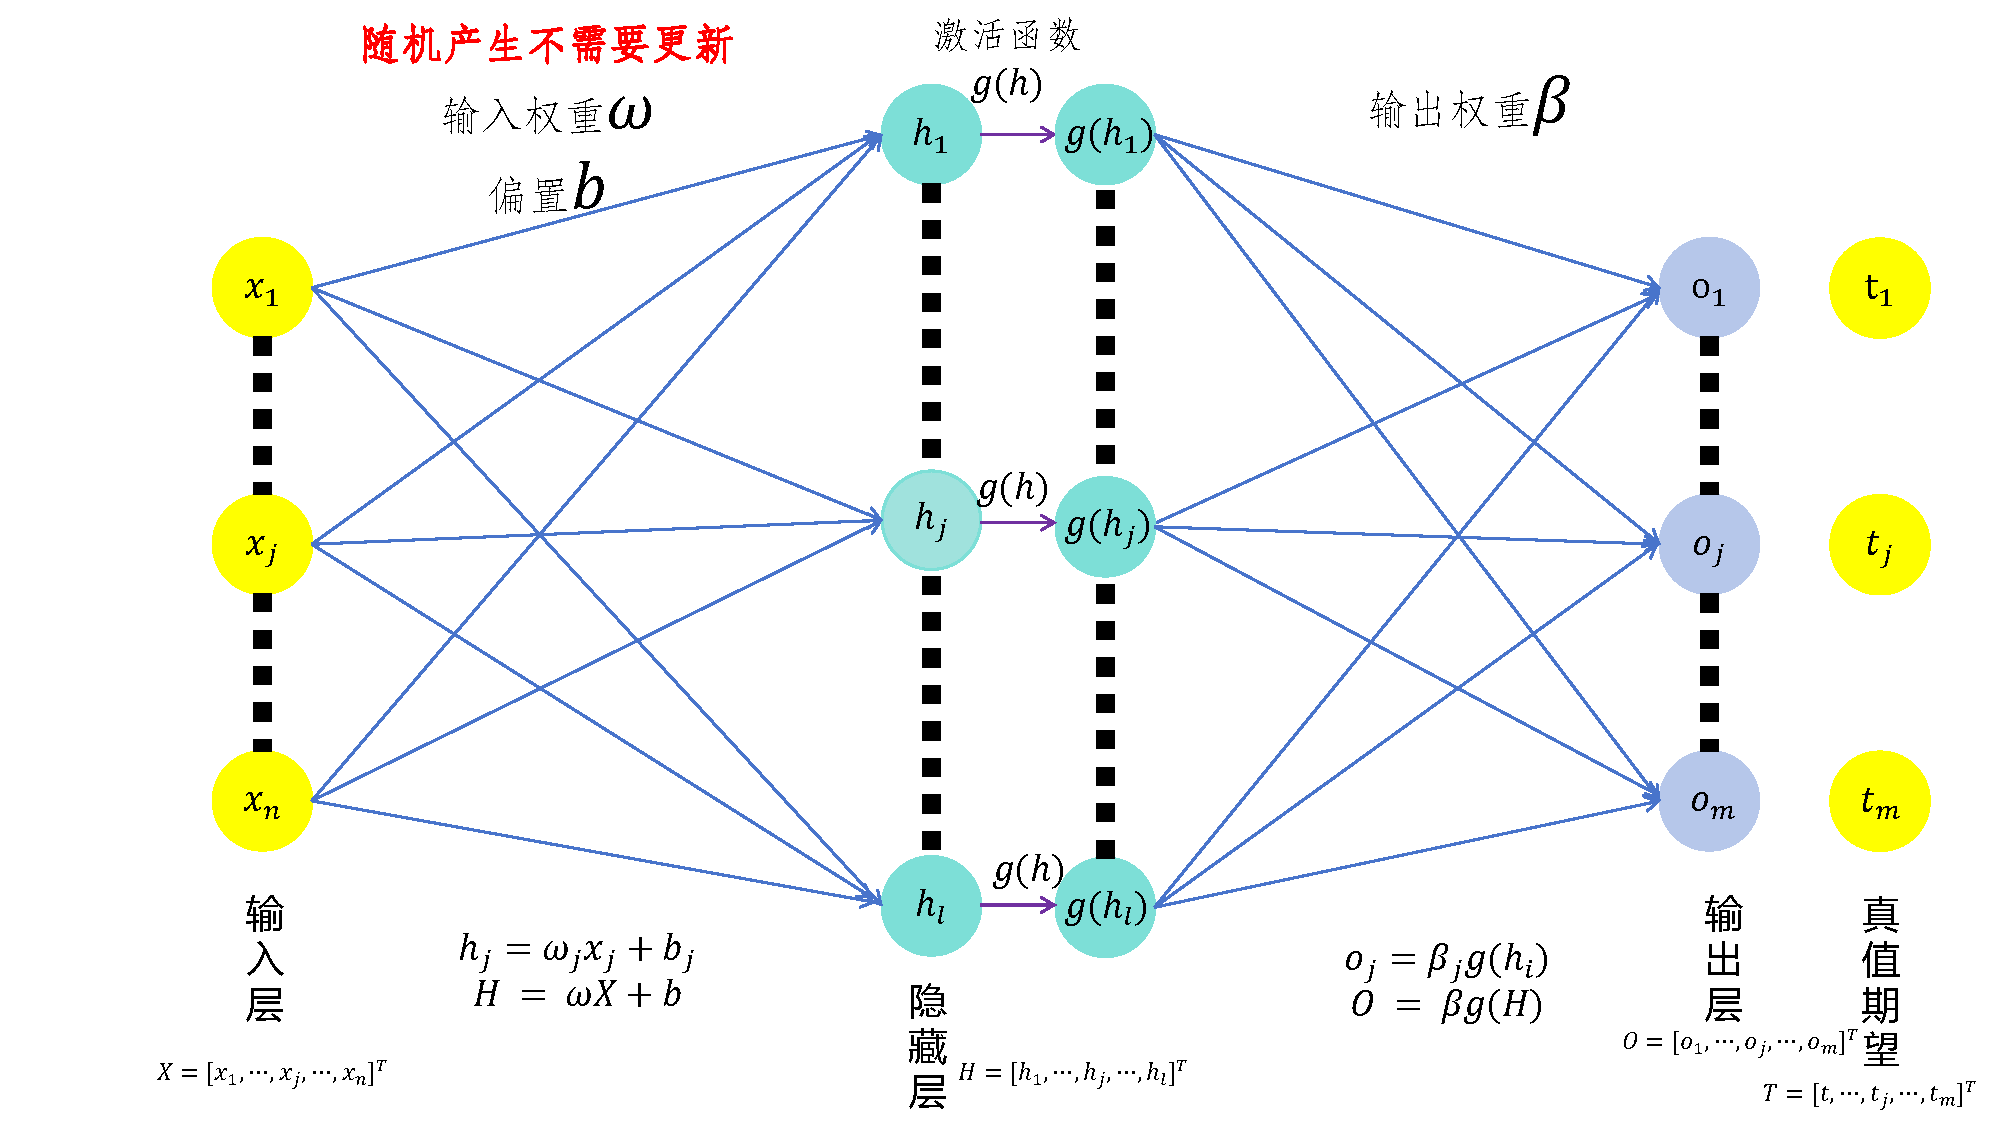
\includegraphics[scale=0.3]{Fig/单隐层前馈神经网络(SLFN).pdf}\\ 
		\hspace{-9em}\scriptsize{Photo source:ZJW's BLOG} 
		\vspace{-0.5em} 
		\caption{SLFN} 
		\label{SLFN} 
	\end{figure}
	
\end{frame}

%----------------------------------------------------------------------------------------
\section{Table}

\linespread{1}  
\begin{frame}{\textbf{Insert Table}}
\linespread{1.5} 

	\begin{table}[htbp]
		\centering 
		\caption{JiLin University Undergraduate Entrance Examination Data Summary (2022/2023)}
		\extrarowheight=2pt 
		\label{loan} 
		\scalebox{0.9}{ 
		\begin{tabular}{p{5cm} p{3cm}<{\centering} p{3cm}<{\raggedleft}} 
			\toprule
			\midrule
 			& 2022 & 2023\\
			\midrule
			Mathematics & 56 & 58 \\
			CS & // & 53 \\
			Artificial Intelligence & 6 & 6 \\
			Software Engineering & 48 & 48 \\
			\midrule
			\bottomrule
		\end{tabular}
		}
		\par\smallskip
		\hspace{2em}\parbox{0.8\textwidth}{\scriptsize 
		Source: \href{https://zsb.jlu.edu.cn/index/examscores.html}{Undergraduate Entrance Examination Data Summary}.\par
		Note: \parbox[t]{0.6\textwidth}{\scriptsize % Remember to be slightly smaller than the first two lines of \textwidth
			You can add notes here.
		}
		}
	\end{table}
	
\end{frame}


%----------------------------------------------------------------------------------------

\linespread{1} 
\begin{frame}{\textbf{Insert Table (Continued)}}
\linespread{1.5} 

	\begin{table}[htbp]
		\centering 
		\caption{The Five Best Industries in the Past Five Years}
		\extrarowheight=2pt 
		\label{CareerCast} 
		\scalebox{0.8}{ 
		\begin{tabular}{@{}crrrr@{}} 
			\toprule
			\midrule
			 Rank & 2021 &  2019 & 2018 & 2017\\
			\midrule
			1 & \textbf{IT Internet} & \textbf{IT Internet}  &  Finance & \textbf{IT Internet} \\
			2 & \textbf{Electronic Semiconductor} & Finance & \textbf{IT Internet}  & Finance \\
			3 & Service Industry & \textbf{Electronic Semiconductor}  & Service Industry & \textbf{Electronic Semiconductor}\\
			4 & Finance & Medical  & \textbf{New Energy} & Real Estate \\
			5 & \textbf{Mechanical Manufacturing} & Service Industry & \textbf{New Energy} & Service Industry \\
			\midrule
			\bottomrule
		\end{tabular}
		}
		\par\smallskip
		\hspace{0.5em}\parbox{0.6\textwidth}{\scriptsize
		Source: ChatGPT, from: \url{https://chat.openai.com}.\par
		Note: \parbox[t]{0.5\textwidth}{\scriptsize
			1. ChatGPT generates answers that are not necessarily correct.\\
		 	2. Bold indicates STEM-related industries.
		}
		}
	\end{table}

\end{frame}

%----------------------------------------------------------------------------------------
\section{Two-column text}
\linespread{1}  
\begin{frame}{\textbf{Two-column text(Or multi-column)}}
\linespread{1.5} 

	\begin{columns}[c]
		\column{0.67\textwidth} 
			\begin{enumerate}[]
				\item We should mention the previous figure, table, or equation in the text as follows:
				\begin{enumerate}[]
					\item [figure $\backslash$ref\{label name\}],
					     it can appear as Figure \ref{SLFN} and Figure \ref{LaTeX}.
					\item [table $\backslash$ref\{label name\}],
						it can appear as Table \ref{loan} and Table \ref{CareerCast}.
					\item [equation $\backslash$ref\{label name\}],
						it can appear as Equation (\ref{reg}) and Equation (\ref{var}).
				\end{enumerate}
				\item The benefits of citation are that when the brief changes, the numbering does not need to be adjusted manually.
			\end{enumerate}

		\column{0.33\textwidth}  
			\begin{figure}
				
\includegraphics[scale=0.045]{Fig/LaTeX.png}\\
				\scriptsize{Source:
				\href{https://en.wikipedia.org/wiki/LaTeX}{Wikipedia}。}\\
				\caption{\LaTeX}
				\label{LaTeX} 
			\end{figure}
	\end{columns}
\end{frame}


%----------------------------------------------------------------------------------------
%	其他
%----------------------------------------------------------------------------------------

\begin{frame}

	Make a new page without a title and display a hyperlink button.
	
	\bigskip
	
	\hyperlink{Linked_text}{\beamergotobutton{Click to jump to the linked text}}
	
\end{frame}

%----------------------------------------------------------------------------------------
\section{Reference}
\linespread{1} 
\begin{frame}{\textbf{The Method of Citing References}}
\linespread{1.5}

	The method of citing references is as follows:
	
	\begin{enumerate}[1]
		\item When using the author of the literature as the subject: \textbackslash citet\{given label\}.
		\item At the end of the text as a supplementary explanation: \textbackslash citep\{given label\}.
	\end{enumerate}
	
	\bigskip

	Take the text as an example:
	
	\begin{enumerate}[1]
		\item \citet{Polynomial_Galerkin} 与 \citet{脉冲微分方程COVID-19}
		\item \citep{Polynomial_Galerkin} 与 \citep{脉冲微分方程COVID-19}
	\end{enumerate}
	
\end{frame}

%----------------------------------------------------------------------------------------

\linespread{1} 
\begin{frame}{\textbf{Reference}}
\linespread{1.5} 

\footnotesize

\begin{thebibliography}{99} 

	\bibitem[JJW (2019)]{Polynomial_Galerkin}
		JJW (2019). 
		\newblock Polynomial preserving recovery for a class of weak Galerkin finite element methods, 
		\newblock \emph{Journal of Computational and Applied Mathematics}, 2019(362), 528-539. 

	\bibitem[贾继伟 (2019)]{脉冲微分方程COVID-19} 
		贾继伟 (2019)。 
		\newblock 基于脉冲微分方程的COVID-19境外输入型病例对我国疫情防控影响的分析:2021年,
		\newblock \emph{中国科学·数学},51(4), 659。
		
\end{thebibliography}

\end{frame}

%----------------------------------------------------------------------------------------
\section*{Closing Slide}
\begin{frame}[plain] % Hides the headline and footline
	\begin{center}
		{\Huge The End}
		
		\bigskip\bigskip 
		
		{\LARGE Questions? Comments?}
	\end{center}
\end{frame}

%----------------------------------------------------------------------------------------

\end{document} 
